%%%%%%%%%%%%%%%%%%%%%%%%%%%%%%%%%%%%%%%%%%%%%%%%%%%%%%%%%%
%                                                                                      %
%         Bristol Project LaTex Template            %
%                                                                                      %
%%%%%%%%%%%%%%%%%%%%%%%%%%%%%%%%%%%%%%%%%%%%%%%%%%%%%%%%%%
%
%   Author: Alex Charles           Email: aep.charles@gmail.com
%
% -----------------------------------------------------------------------------------
%      PACKAGES & OTHER DOCUMENT CONFIGURATIONS
% -----------------------------------------------------------------------------------
\documentclass[11pt]{article}
\usepackage[utf8]{inputenc}
\usepackage[T1]{fontenc}
\usepackage[british]{babel}
% ----------NEW BIBLATEX BIBLIOGRAPHY-----------------------------------------------
\usepackage[backend=bibtex,style = ieee]{biblatex} % Upgrades Bibliography

\addbibresource{BibFile.bib} %%% For biblatex
%e.g to add page number \footfullcite[chapter, p.~215]{AAIB}
% This allows can use footfullcite commands
% Note urldate field must be in yyyy-mm-dd to work - use online type
% Remeber to use \printbibliography in the footer
% -----------------------------------------------------------------------------------
\usepackage{sectsty}
\usepackage{amssymb,amsmath}
\usepackage{ifxetex,ifluatex}  %<<<<<<<<< Edit FONT HERE
\ifnum 0\ifxetex 1\fi\ifluatex 1\fi=0 % if pdftex
  \usepackage[T1]{fontenc}
  \usepackage[utf8]{inputenc}
\else % if luatex or xelatex
  \ifxetex
    \usepackage{mathspec}
    \setmainfont{Avenir-Light}
  \else
  % Font Package for XeLatex
    \usepackage{fontspec}
    \setmainfont{Avenir-Light}
  \fi
  \defaultfontfeatures{Ligatures=TeX,Scale=MatchLowercase}
\fi
\usepackage[fit]{truncate} %Truncates headers that are too long
\usepackage{fancyhdr}
\usepackage{lastpage}
\usepackage{extramarks}
\usepackage{gensymb}
\usepackage{lipsum}
\usepackage{float}
\usepackage{graphicx}
\graphicspath{{TempImg/}{Img/}}%<<<<<<<<< Location of Template Images and Other Images, Add folders here
\usepackage{subfig}
\usepackage{wrapfig}
\usepackage[font ={small,it}]{caption}
\usepackage{amsfonts,amsthm} % Math packages
% \usepackage{cite}
% \usepackage[maxlevel=3]{csquotes}
%    \MakeAutoQuote{‘}{’}
%    \MakeAutoQuote*{“}{”} %corrects quote marks
\usepackage{enumitem} % resume numbered lists
\usepackage{multicol} %for mulitple colums in lists
\usepackage{geometry}
\usepackage{booktabs} %<<<<<<<<< Table drawing package
\usepackage[table,xcdraw]{xcolor} %<<<<<<<<< Table drawing package
\usepackage{svg}
\usepackage{scrextend} %call footnotes
\usepackage[colorlinks, linkcolor = black, citecolor = black, filecolor = black, urlcolor = blue]{hyperref} % Creates Hyperlinks for references - add [colorlinks] for coloured hyperlinks
\usepackage{changepage} %Allows Adjust width to be used for the document (indenting paragraphs)
\usepackage{pdfpages} %Allows Pdfpages to be added to the document use \includepdf[pages={1}]{myfile.pdf}
\usepackage{pdflscape} %Change Pages from Portrait to Landscape

%\usepackage[compact]{titlesec}
\usepackage{titlesec}
\titlespacing\section{0pt}{2pt plus 2pt minus 2pt}{0pt plus 2pt minus 2pt}
\titlespacing\subsection{0pt}{0pt plus 3pt minus 2pt}{-3pt plus 2pt minus 2pt}
\titlespacing\subsubsection{0pt}{0pt plus 2pt minus 2pt}{-4pt plus 2pt minus 2pt}
\titlespacing\subsubsubsection{0pt}{-6pt plus 2pt minus 2pt}{-4pt plus 2pt minus 2pt}
\setlength{\multicolsep}{-1pt plus 2.0pt minus 1.5pt}% 50% of original values

% \titlespacing*{\section}{0pt}{1.1\baselineskip}{\baselineskip}

\renewcommand*{\thefootnote}{\alph{footnote}} %%% Changes footnotes to letters
\usepackage[bottom]{footmisc} %%% Pushes footnote to bottom and to the margin

\DeclareCiteCommand{\footcite}[\mkbibfootnote]
{\usebibmacro{cite:init}%
\usebibmacro{prenote}}
{\usebibmacro{citeindex}%
\printtext[brackets]{\usebibmacro{cite:comp}}}
{\multicitedelim}
{\usebibmacro{cite:dump}%
\usebibmacro{postnote}}

\newenvironment{indentpara}{\begin{adjustwidth}{2cm}{}}{\end{adjustwidth}} %Declare adjust width wiht indentpara
\renewcommand{\labelitemii}{$\circ$}
\renewcommand{\labelitemiii}{$\diamond$}
\renewcommand{\labelitemiii}{$\cdot$}

% -----------------------------------------------------------------------------------
%                 Code
% -----------------------------------------------------------------------------------
\usepackage{listings}
\lstset{inputpath=Code/}
\usepackage{color}
\definecolor{mygreen}{RGB}{28,172,0} % color values Red, Green, Blue
\definecolor{mylilas}{RGB}{170,55,241}

\lstset{language=Matlab,%
    %basicstyle=\color{red},
    breaklines=true,%
    basicstyle=\small,
    morekeywords={matlab2tikz},
    keywordstyle=\color{blue},%
    morekeywords=[2]{1}, keywordstyle=[2]{\color{black}},
    identifierstyle=\color{black},%
    stringstyle=\color{mylilas},
    commentstyle=\color{mygreen},%
    showstringspaces=false,%without this there will be a symbol in the places where there is a space
    numbers=left,%
    numberstyle={\tiny \color{black}},% size of the numbers
    numbersep=9pt, % this defines how far the numbers are from the text
    emph=[1]{for,end,break},emphstyle=[1]\color{red}, %some words to emphasise
    %emph=[2]{word1,word2}, emphstyle=[2]{style},
}

%% To Add Code Use :
% \lstinputlisting{myfun.m}
%% To input a file or :
% \begin{figure}[h]
% \begin{lstlisting}[language=Matlab]
% \end{lstlisting}
% \catpion{code}
% \end{figure}


% -----------------------------------------------------------------------------------
%                 Quotes
% -----------------------------------------------------------------------------------

\usepackage{epigraph}
% \epigraphsize{\small}% Default
\setlength\epigraphwidth{12cm}
\setlength\epigraphrule{0pt}

\usepackage{etoolbox}
\apptocmd{\sloppy}{\hbadness 10000\relax}{}{}%%%% > Removes Url bibliography warnings
\makeatletter
\patchcmd{\epigraph}{\@epitext{#1}}{\itshape\@epitext{#1}}{}{}
\makeatother

%%%% > For Quotes Use \epigraph{"Quote"}{ - \textup{Author}, Book}

% -----------------------------------------------------------------------------------
%                   NAMES & CLASS DEFINITION %<<<<<<<<< INSERT DETAILS HERE
% -----------------------------------------------------------------------------------
\newcommand{\AssignmentTitle}{Part 2: Elevation Axis– Theory and Simulation with Control Requirements}
\newcommand{\ModuleTitle}{Sensors, Signals and Control}
\newcommand{\University}{University of Bristol}
\newcommand{\Faculty}{Faculty of Engineering}
\newcommand{\UniCrest}{crestbris.png}
\newcommand{\UniLogo}{logobris.png}%<<<<<<<<< Make Sure Files are in the Template
%\newcommand{\GroupName}{Group 2}
\newcommand{\StudentNameA}{Alex Charles}
\newcommand{\StudentNumberA}{ac13625}
\newcommand{\StudentNameB}{Akash Ramineni}
\newcommand{\StudentNumberB}{ar14120}
\newcommand{\SupervisorNameA}{Andres Marcos}
\newcommand{\SupervisorEmailA}{Andres.Marcos@bristol.ac.uk}
\newcommand{\SupervisorNameB}{Name}
\newcommand{\SupervisorEmailB}{email@gmail.com}

% -----------------------------------------------------------------------------------
%        PACKAGES FOR MARKDOWN CONVERSION - FOR USE If Using Markdown to Latex
% -----------------------------------------------------------------------------------
\usepackage{fixltx2e} % provides \textsubscript
% use upquote if available, for straight quotes in verbatim environments
\IfFileExists{upquote.sty}{\usepackage{upquote}}{}
% use microtype if available
\IfFileExists{microtype.sty}{%
\usepackage{microtype}
\UseMicrotypeSet[protrusion]{basicmath} % disable protrusion for tt fonts
}{}
\hypersetup{unicode=true,
            pdftitle={\AssignmentTitle},
            pdfauthor={\StudentNameA},
            pdfborder={0 0 0},
            breaklinks=true}
\urlstyle{same}  % don't use monospace font for urls
\usepackage{fancyvrb}
\VerbatimFootnotes % allows verbatim text in footnotes
\usepackage{longtable,booktabs}
\IfFileExists{parskip.sty}{%
\usepackage{parskip}
}{% else
\setlength{\parindent}{0pt}s
\setlength{\parskip}{6pt plus 2pt minus 1pt}
}
\setlength{\emergencystretch}{3em}  % prevent overfull lines
\providecommand{\tightlist}{%
  \setlength{\itemsep}{0pt}\setlength{\parskip}{0pt}}
% \setcounter{secnumdepth}{0}
% Redefines (sub)paragraphs to behave more like sections
\ifx\paragraph\undefined\else
\let\oldparagraph\paragraph
\renewcommand{\paragraph}[1]{\oldparagraph{#1}\mbox{}}
\fi
\ifx\subparagraph\undefined\else
\let\oldsubparagraph\subparagraph
\renewcommand{\subparagraph}[1]{\oldsubparagraph{#1}\mbox{}}
\fi

% -----------------------------------------------------------------------------------
%                   WORD COUTNER - for XeLaTex
% -----------------------------------------------------------------------------------
\usepackage{xesearch}
\newcounter{words}
\newenvironment{counted}{%
  \setcounter{words}{0}
  \SearchList!{wordcount}{\stepcounter{words}}
    {a?,b?,c?,d?,e?,f?,g?,h?,i?,j?,k?,l?,m?,
    n?,o?,p?,q?,r?,s?,t?,u?,v?,w?,x?,y?,z?}
  \UndoBoundary{'}
  \SearchOrder{p;}}{%
  \StopSearching}

% -----------------------------------------------------------------------------------
%                   MARGINS, HEADERS & FOOTERS
% -----------------------------------------------------------------------------------
 \geometry{
 left=20mm,
 right=20mm,
 top=20mm,
 bottom=20mm,
 }
\linespread{1.05}

\pagestyle{fancy}
\lhead{\includegraphics[width = 0.2\textwidth]{\UniLogo}}
% \chead{\AssignmentTitle}
% \rhead{}
\lfoot{\StudentNameA, \StudentNameB}
\cfoot{}
\rfoot{Page \thepage} %%%% note the footer is swapped when page numbering style changes
\renewcommand\headrulewidth{0.4pt}
\renewcommand\footrulewidth{0.4pt}

\setlength\parindent{0pt}

\newcommand{\horrule}[1]{\rule{\linewidth}{#1}}

% -----------------------------------------------------------------------------------
%               DOCUMENT STRUCTURE COMMANDS
% -----------------------------------------------------------------------------------
% To sort out the formatting of header and footer when a page...
% ... split occurs "within" a problem environment.
\newcommand{\enterProblemHeader}[1]{
\nobreak\extramarks{#1 (Cont.)}\nobreak
\nobreak\extramarks{#1}{}\nobreak
}
% To sort out the formatting of header and footer when a page...
% ... split occur "between" problem environments.
\newcommand{\exitProblemHeader}[1]{
\nobreak\extramarks{#1 (Cont.)}\nobreak
\nobreak\extramarks{#1}{}\nobreak
}

% -----------------------------------------------------------------------------------
\begin{document}

  \setlength{\abovedisplayskip}{-14pt}
  \setlength{\belowdisplayskip}{2pt}
  \setlength{\abovedisplayshortskip}{-14pt}
  \setlength{\belowdisplayshortskip}{2pt}

  \setlist[enumerate]{itemsep=-2mm}
  \setlist[itemize]{itemsep=-2mm}


%----------------------------------------------------------------------------------------
                                  %	TITLE PAGE FORMAT
%----------------------------------------------------------------------------------------
\pagenumbering{roman}
\begin{titlepage}

	\center % Center everything on the page
%----------------------------------------------------------------------------------------
%	HEADING SECTION
%----------------------------------------------------------------------------------------
		\usefont{OT1}{bch}{b}{n}
		\normalfont \normalsize \textsc{\University} \\ [10pt]
		\normalfont \normalsize \textsc{\Faculty} \\ [25pt]
%----------------------------------------------------------------------------------------
%	LOGO SECTION - Adds Univeristy Crest to the Report
%----------------------------------------------------------------------------------------
		\includegraphics[width = 0.2\textwidth]{\UniCrest}\\[0.5cm]
%----------------------------------------------------------------------------------------
%	HEADING SECTION
%----------------------------------------------------------------------------------------
		\normalfont \normalsize \textsc{\ModuleTitle} \\ [25pt]
%----------------------------------------------------------------------------------------
%	TITLE SECTION
%----------------------------------------------------------------------------------------
		\horrule{0.5pt} \\[0.4cm]
		\huge \textbf{\AssignmentTitle} \\
		\horrule{2pt} \\[0.5cm]
%----------------------------------------------------------------------------------------
%	HEADING SECTION
%----------------------------------------------------------------------------------------
%		\normalfont \normalsize \textsc{\GroupName} \\ [25pt]
%----------------------------------------------------------------------------------------
%	AUTHOR SECTION
%----------------------------------------------------------------------------------------
\begin{minipage}{0.4\textwidth}
\begin{flushleft} \large
\emph{Supervisors:}\\
% Change Name
\textbf{\SupervisorNameA}\\
% \textbf{\SupervisorNameB}
\end{flushleft}
\end{minipage}
~
\begin{minipage}{0.4\textwidth}
\begin{flushright} \large
\emph{Email:} \\
\SupervisorEmailA\\
% \SupervisorEmailB

\end{flushright}
\end{minipage}\\[1cm]

\begin{minipage}{0.4\textwidth}
\begin{flushleft} \large
\emph{Authors:}\\
	\textbf{\StudentNameA}\\
  \textbf{\StudentNameB}
\end{flushleft}
\end{minipage}
~
\begin{minipage}{0.4\textwidth}
\begin{flushright} \large
\emph{Candidate Number:} \\
(\StudentNumberA)\\
(\StudentNumberB)
\end{flushright}
\end{minipage}\\[2cm]

%----------------------------------------------------------------------------------------
%	DATE SECTION
%----------------------------------------------------------------------------------------
\textit{{\large \today}}\\[1cm] % Date, change the \today to a set date if you want to be precise
%----------------------------------------------------------------------------------------
\vfill % Fill the rest of the page with whitespace
\end{titlepage}

% \setcounter{page}{3}

\newpage


% -----------------------------------------------------------------------------------
%                             	 ABSTRACT
% -----------------------------------------------------------------------------------

% \addcontentsline{toc}{section}{Abstract}
% \begin{abstract}
%
% \end{abstract}
% -----------------------------------------------------------------------------------
%                              TABLE OF CONTENTS
% -----------------------------------------------------------------------------------

% \tableofcontents


% \newpage

% \addcontentsline{toc}{section}{List of Tables}
% \listoftables
% \addcontentsline{toc}{section}{List of Figures}
% \listoffigures
% \addcontentsline{toc}{section}{List of Acronyms}
% \section*{List of Acronyms}\label{acronyms}
% \textbf{BRB}: Be Right Back \\


% \newpage

% \addcontentsline{toc}{section}{Acknowledgements}
% \section*{Acknowledgements}\label{acknowledgements}

% \addcontentsline{toc}{section}{Declaration}
% \section*{Declaration}\label{declartion}
% I hereby declare that this report entitled “\AssignmentTitle” submitted to Bristol University, is a record of an original work completed by myself.\\

% \newpage

%% -----------------------------------------------------------------------------------
%%                          	  INTRODUCTION
%% -----------------------------------------------------------------------------------
\clearpage
\rfoot{Page \thepage\ of \pageref{LastPage}}
\pagenumbering{arabic}
\begin{counted} %<<<<<<<<<<<<<<STARTS WORD COUNTER
\section{P-I-D analysis}\label{p-i-d-analysis}

This report introduces the effects of proportional, derivative and
integral terms for a typical PID controller. The effect of varying gain
is assessed using time-domain and root locus results. For a closed loop
classical PID controller, the basic aim is to reduce tracking error
between the control input and the observed output. In an engineering
context, it is desirable to have a sharp response to user input and
correctly tuned PIDs will achieve this. The responses highlighted in
this report are in relation to the Quanser behaviour observed in Control
Coursework Part 1.

\subsection{Proportional Feedback
Controller}\label{proportional-feedback-controller}

\begin{wrapfigure}{l}{0.5\textwidth}
\centering
\vspace{-15pt} % Space added to the top of the image
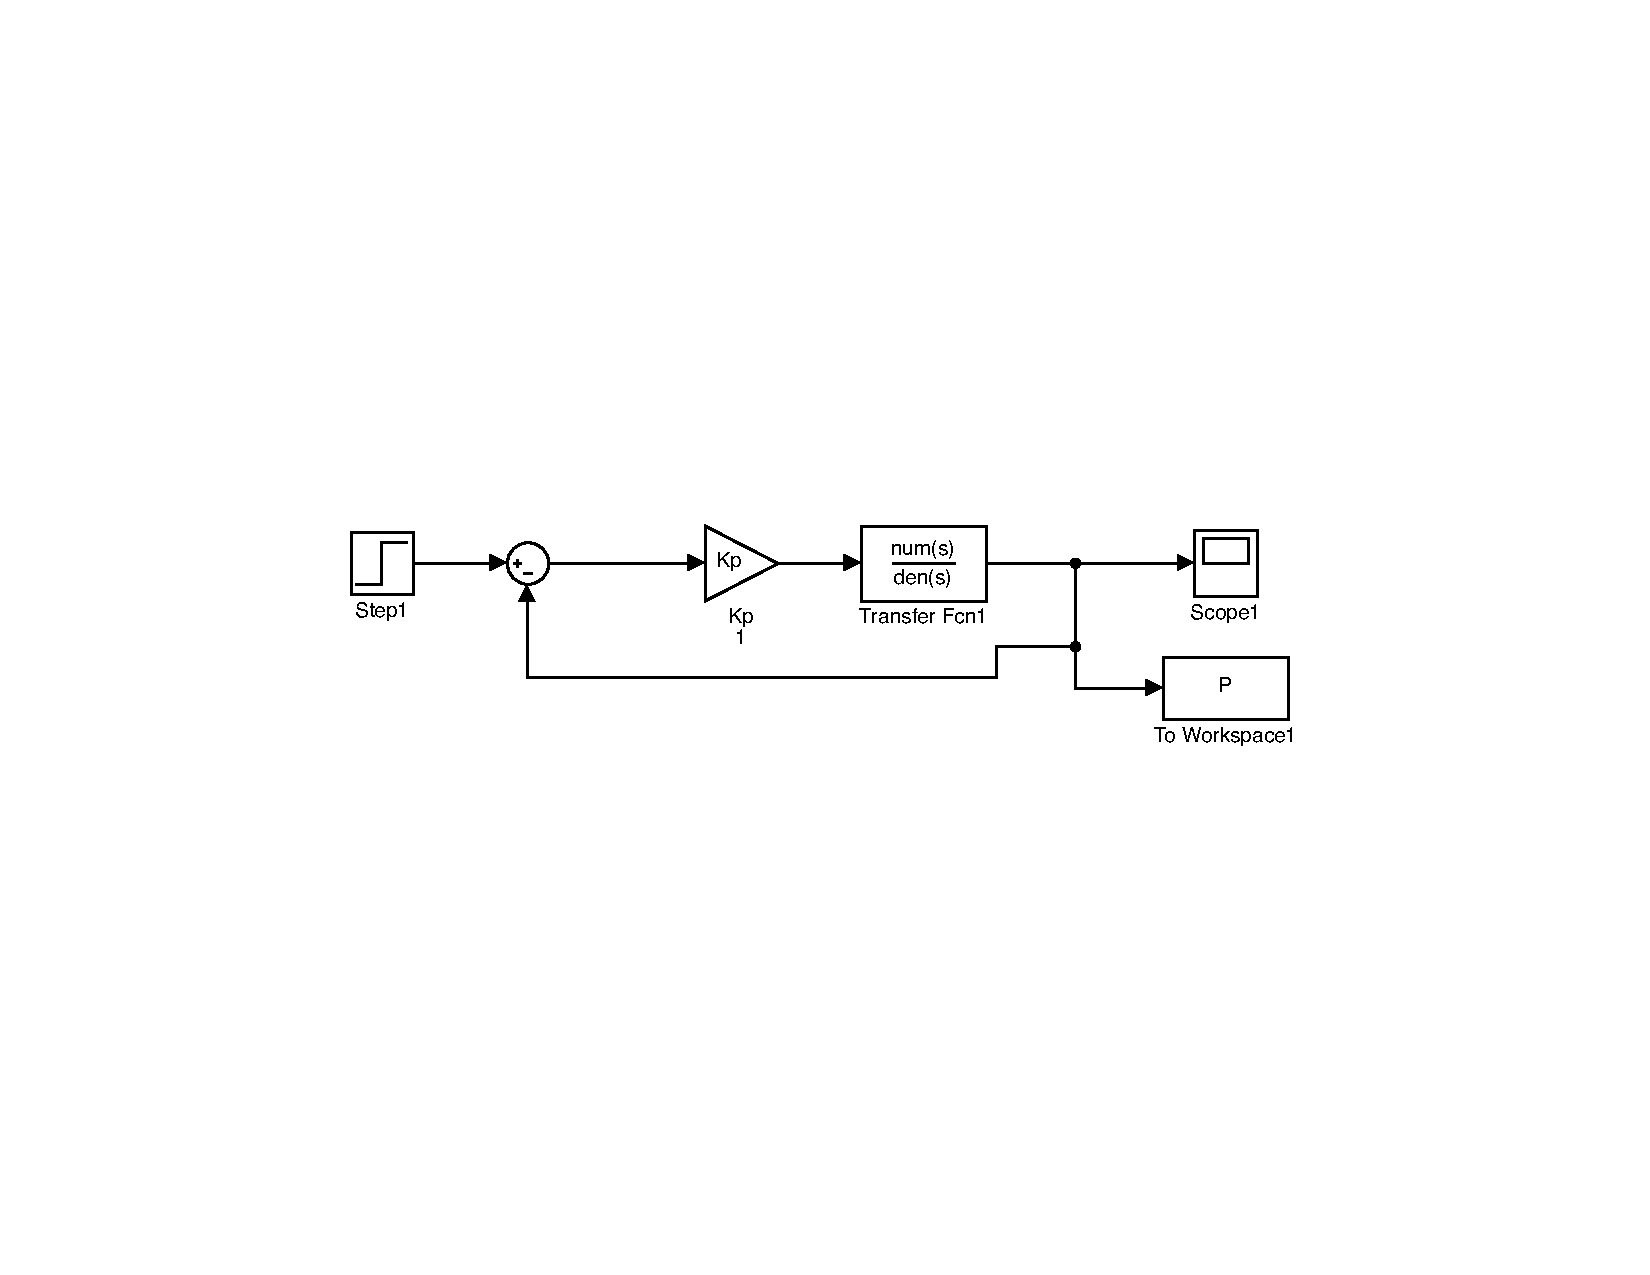
\includegraphics[trim = 0 0 0 0, clip, width=0.5\textwidth]{Psim.pdf}
\vspace{-10pt}
\caption{Caption Text}
\label{Psim}
\vspace{-15pt}
\end{wrapfigure}

Proportional control uses the `Present' state of the plant to error
correct. The correction applied is proportional to the deviation from
the desired state of the plant. This implies a highly oscillatory system
response, as the present error doesn't take into account the past or
future but rather the instantaneous state of the plant. The effect of
varying proportional gain (Kp) was observed through the simulation built
in REFERENCE. This simulation was executed in an iterative loop with
varying Kp from 0 to 0.1 in increments of 0.01. REFERENCE shows the time
domain response of increasing Kp. When Kp = 0, a flat line is observed
as there is no signal passing through the plant. With increasing
proportional gain, the correction factor becomes larger and as seen by
the increased amplitude for higher Kp gains. The `stepinfo()' function
shows that increasing Kp -- reduces rise time and steady state error
whilst increasing overshoot.

The root locus plot in REFERENCE allows observation of s-domain features
with varying proportional gain. For pure variation in proportional gain,
the (stable) poles are restricted to the same distance from the
imaginary axis. In addition, increasing Kp moves the poles away from the
real axis in both directions. This implies increased natural frequency
with increased Kp and decreased damping ratio. This verifies the
observation noted in the time domain plot, as increased natural
frequency will lead to greater oscillatory behaviour and decreased
damping ratio increases the overshoot.

\begin{figure}[H]
\centering
\begin{minipage}{.455\textwidth}
 \centering
 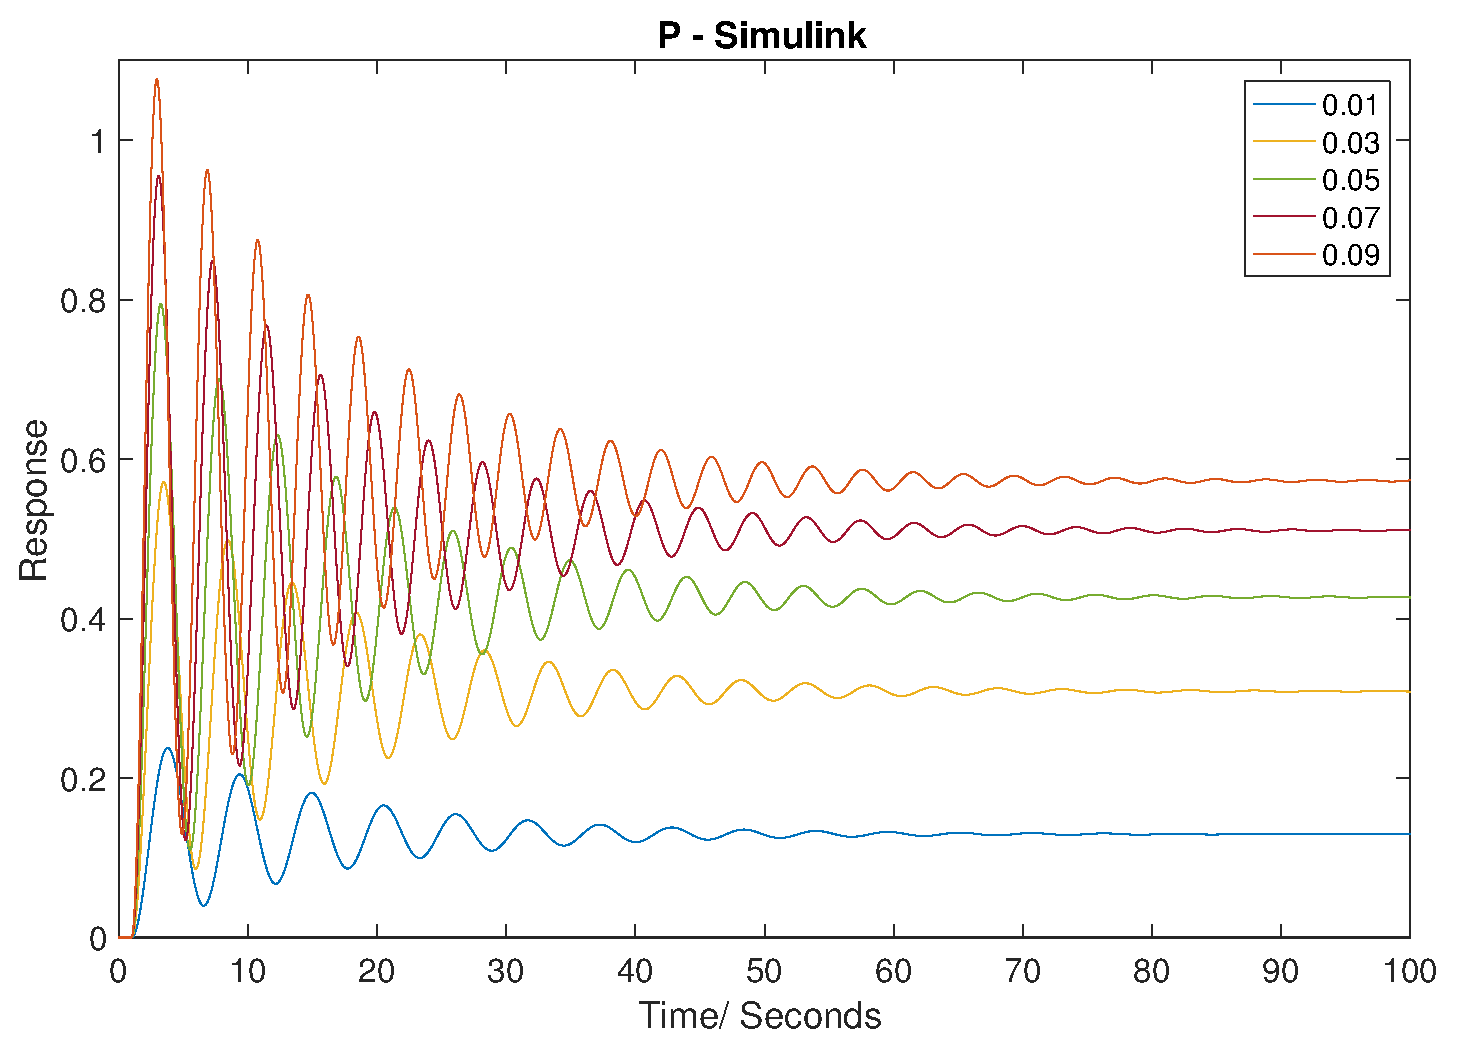
\includegraphics[trim = 0 0 0 0, clip, width=1\textwidth]{pres.eps}
 \caption{}
 \label{pres}
\end{minipage}
\hfill
\begin{minipage}{.455\textwidth}
\centering
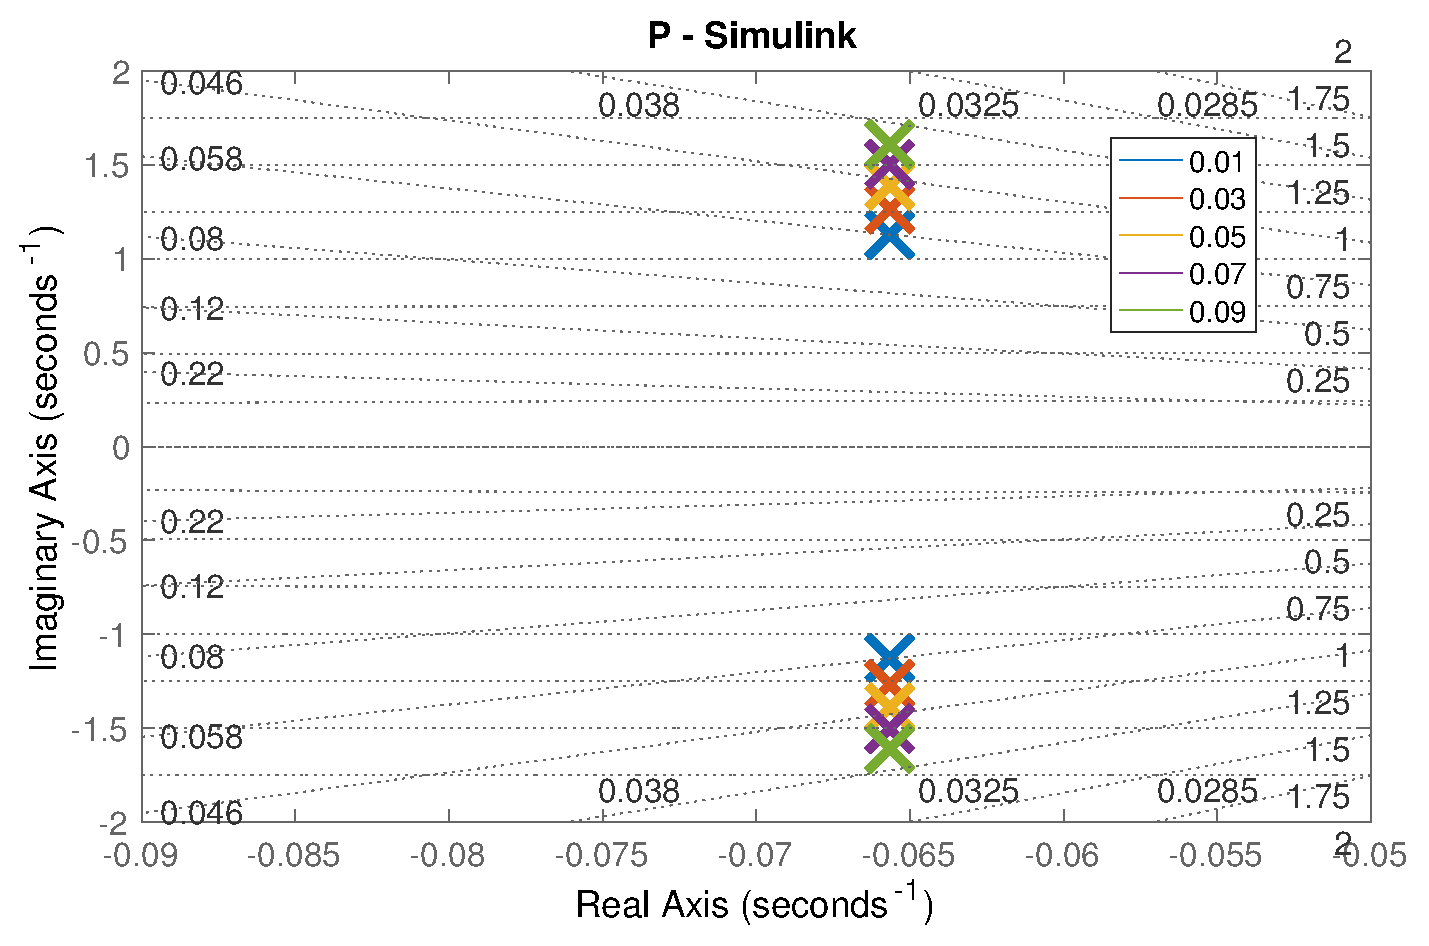
\includegraphics[trim = 0 0 0 0, clip, width=1\textwidth]{pzp.eps}
\caption{}
\label{pzp}
\end{minipage}
\vspace{-20pt}
\end{figure}

\subsection{Derivative Feedback
Controller}\label{derivative-feedback-controller}

\begin{wrapfigure}{l}{0.5\textwidth}
\centering
\vspace{-15pt} % Space added to the top of the image
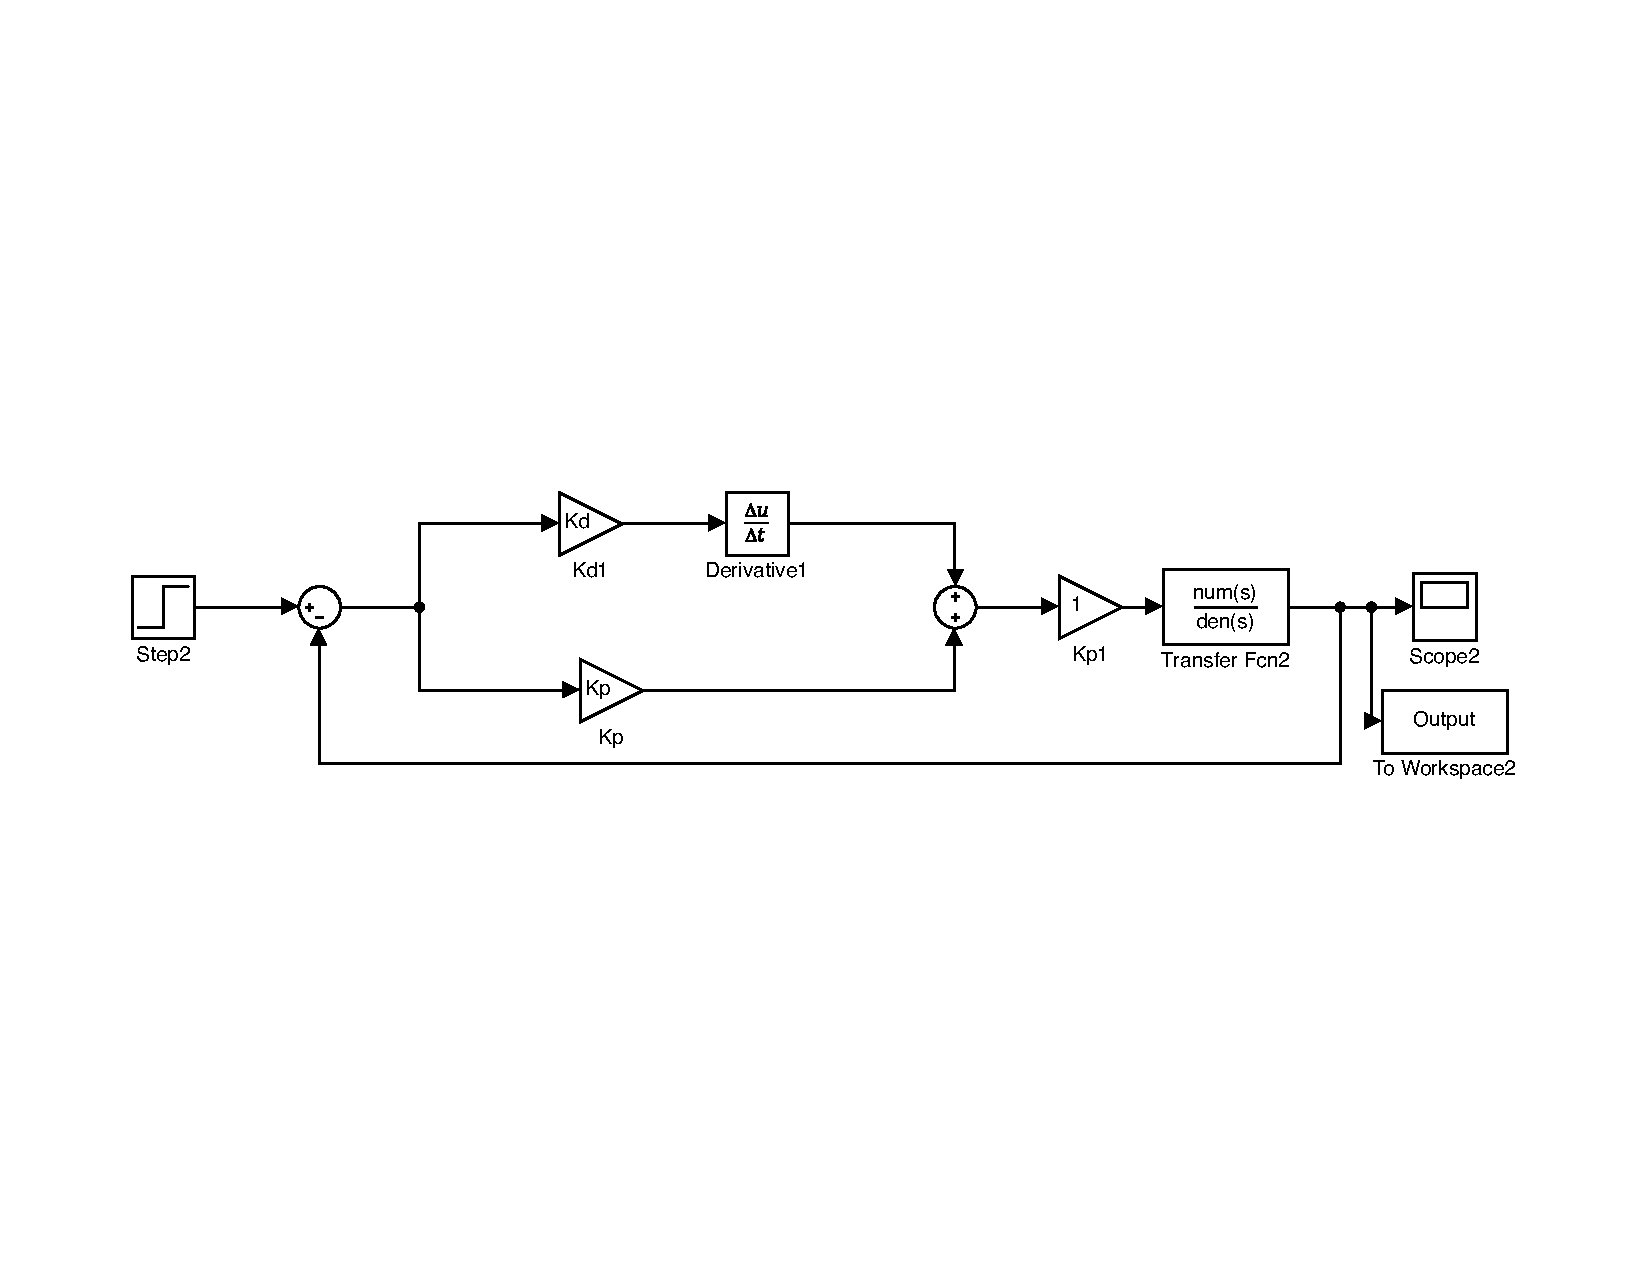
\includegraphics[trim = 0 0 0 0, clip, width=0.5\textwidth]{pd2.pdf}
\vspace{-10pt}
\caption{Caption Text}
\label{pd2}
\vspace{-15pt}
\end{wrapfigure}

Derivative control utilises the expected `Future' state of the system to
pre-emptively produce an error correct signal. This correction is
proportional to the rate of change of the system state at a point in
time. The system calculates the state of the plant in the future based
on rate of change conditions correctly and accounts for that by
anticipating the response. For this reason a large damping effect is
expected for increasing derivative gain (Kd). The simulation in
REFERENCE was implemented to observe two things -- first the effect of
purely varying derivative gain with constant proportional gain, and
second the effect of varying both gains by the same amount -- this was
controlled using the additional gain block after the controller. The
gain/s in both REFERENCE and REFERENCE was incremented from 0 to 1 in
increments of 0.05.

As expected, the time domain responses show that increasing Kd has a
greater damping effect on oscillations. There is a reduction in
overshoot and increase in rise time. For a Kd = 0 , large oscillations
are observed and decrease with increasing gain. For larger gain values
of 0.6 and above there is high damping with the response settling to a
steady level quickly. Increasing both Kd and Kp by the same amount shows
reduction in rise time, overshoot and steady state error. PD control
appears more effective.

The root locus S-domain metrics show that as Kd is increased the poles
are shifted more negatively in the real axis. The semi-circular shape
represents the line of equal proportional gain and points represent
varying Kd at that Kp level. As Kd increases the angle between the
imaginary axis increases -- this implies poles closer to the real axis,
ie higher Kd corresponding poles have greater damping; natural frequency
is reduced (and hence less oscillatory behaviour).

\subsection{Integral Action}\label{integral-action}

\begin{wrapfigure}{l}{0.5\textwidth}
\centering
\vspace{-15pt} % Space added to the top of the image
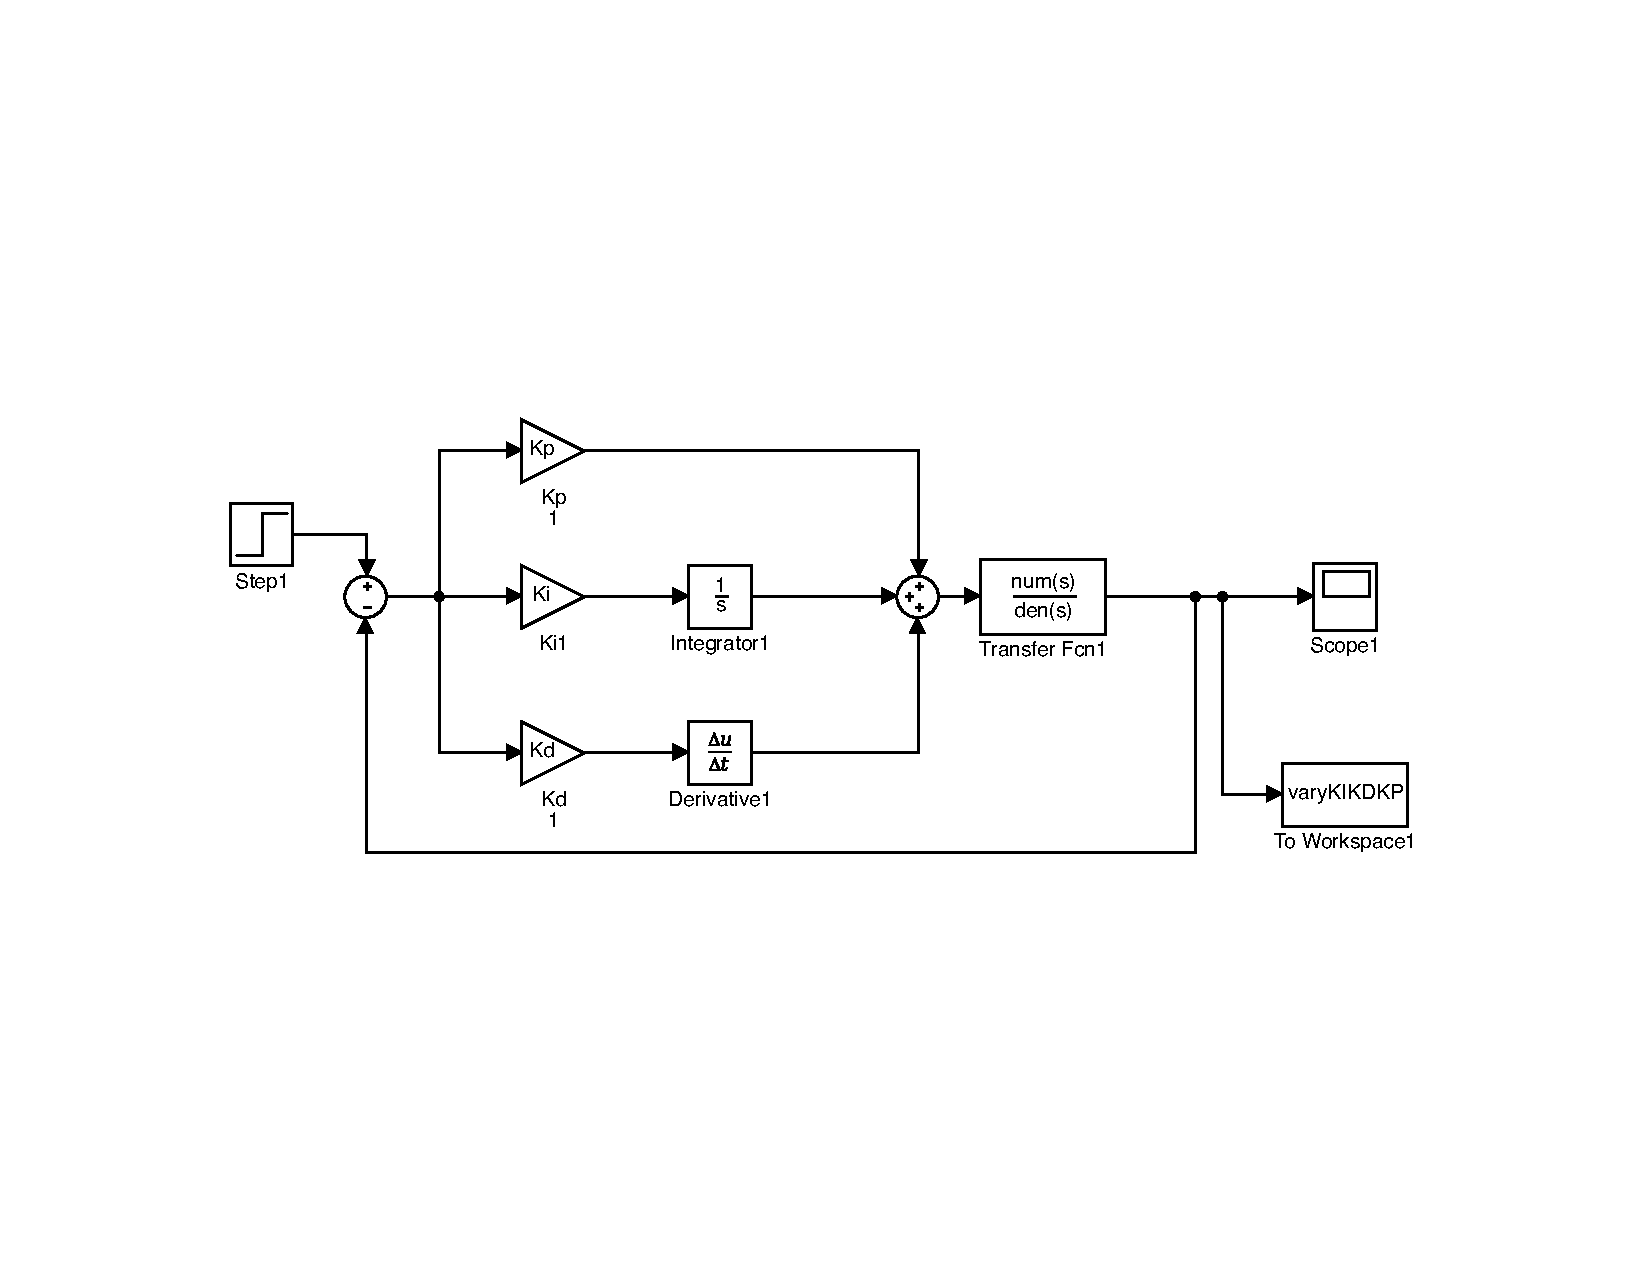
\includegraphics[trim = 0 0 0 0, clip, width=0.5\textwidth]{PIDp2.pdf}
\vspace{-10pt}
\caption{Caption Text}
\label{PIDp2}
\vspace{-15pt}
\end{wrapfigure}

Integral control utilises the `Past' state of the system to produce an
error-correcting signal. The integral term looks at the period and how
far the measured variable is from the desired state in time. This
controller sums the complete error in history up to current time state.
For this reason the integral control will eliminates offset and leads to
zero steady state error. REFERENCE shows the variation of pure Ki with
constant Kp and Kd. REFERENCE shows the variation of all three gains Kd,
Ki and Kp by the same magnitude -- this was implemented using a
gain-scaling block after the controller. The time domain plots confirm
the zero steady state error as the oscillations level to desired
response level.

0 there is steady state error that exists in the system, but as integral
gain increases the steady state error is completely eliminated. The
preferred controller is PID.

\section{PID Design to Achieve Control
Requirements}\label{pid-design-to-achieve-control-requirements}

\subsection{Open Loop Transfer Function PID
Controller}\label{open-loop-transfer-function-pid-controller}

\subsection{Tuned Quanser Controller}\label{tuned-quanser-controller}
% -----------------------------------------------------------------------------------
%                                  APENDIX
% -----------------------------------------------------------------------------------

\end{counted} %<<<<<<<<<<<<<<ENDS WORD COUNTER

% \newpage
% % \section{Appendices}
% Above were \thewords\ words. %<<<<<<<<<<<<<<DISPLAYS WORD COUNTER
% -----------------------------------------------------------------------------------
%                               BIBLIOGRAPHY - Insert Name of BIB File Here
% -----------------------------------------------------------------------------------
% \newpage

% ---------------BIBTEX OLD-----------------------------------------------------
% \bibliographystyle{unsrt} %%%% Plain or alpha can change orders here
% \bibliography{BibFile}
% \nocite{*} %%%if you want to see all references even those note cited in the text
% -----------------------------------------------------------------------------------

\printbibliography

\end{document}
